%!TEX root=restructured.tex

\begin{figure*}[h!]
  \centering
  \subfloat[overview of the tracked endpoints]{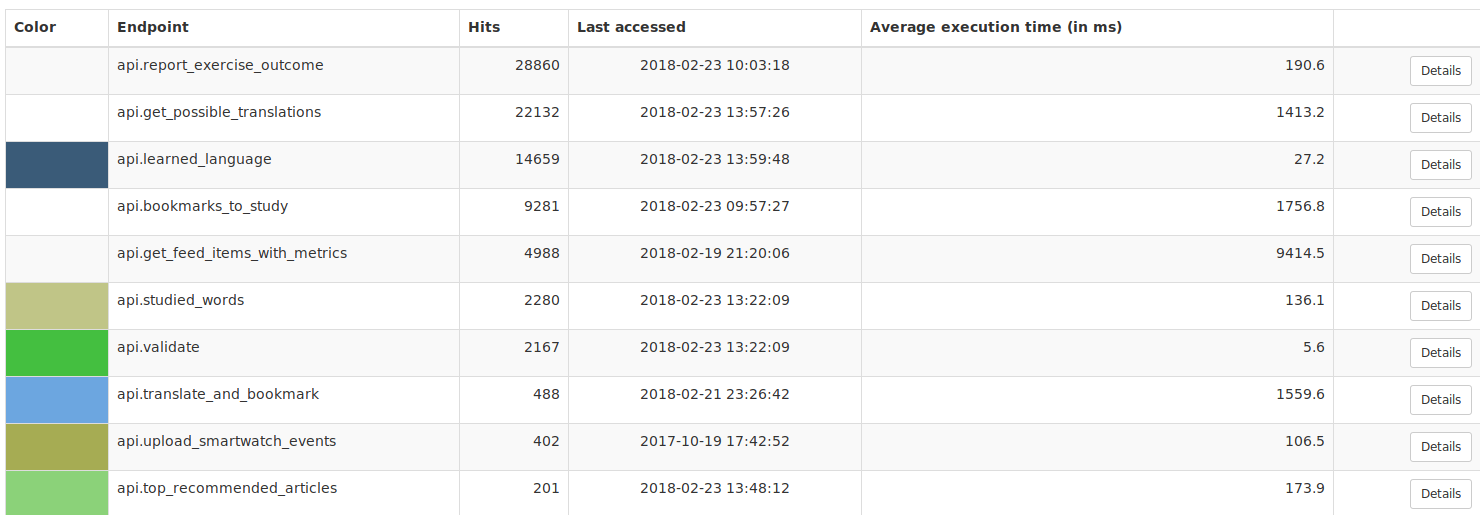
\includegraphics[width=1.5\columnwidth]{overview}\label{fig:overview}}
  \caption{Some of the available views\label{fig:views}}
\end{figure*}



  \newpage
  \section{Evolution monitoring }
  

  When thinking about performance, 
  one can not avoid thinking about the performance evolution. 

  Version control in \tool can be supported in two ways,
  the developer explicitly states the current version, 
  or the current version is automatically detected based
  on some version control system. 


  However, with the current configuration of the tool, it would be impossible for the maintainer to see the improvements resulting from the optimization. 

  \ins{The latest STack Overflow Developer Survey: 88.4\% of **professional** developers use git.}  
  If assume that the code that they run is deployed using .git, then with an extra line of configuration they can allow \tool to find the git\footnote{\url{https://git-scm.com/}} folder of the deployed service and automatically detect the version of the project that is running: 
    
    \begin{lstlisting}[style=custompython]
    
      dashboard.config.git = 'path/to/.git'
      
    \end{lstlisting}  
 
  If the \tool can automatically detect the current version of the project by reading the .git configuration as soon as the API is started and can then group measurements by version\footnote{Alternatively, the maintainer can add version identifiers manually for the web application through a configuration file if the system does not use git.}. \Fref{fig:tee} is a zoomed-in version of such a view for \epTranslations with versions increasing from top to bottom
  
  \begin{figure}[h!]
  \centering
  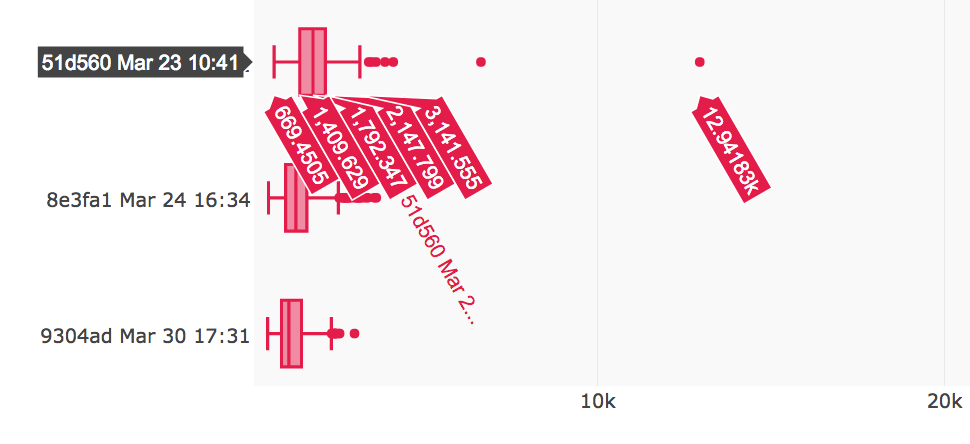
\includegraphics[width=0.9\linewidth]{translation_endpoint_evolution_}
  \caption{The Performance Evolution of the \epTranslations endpoint}
  \label{fig:tee}
\end{figure}


  This view confirms that the performance of the translation endpoint improved in the recent versions: the median of the last three versions is constantly moving towards the left, and progresses from 1.4 seconds (in the top-most box plot in \Fref{fig:tee}) to 0.8 in the latest version (bottom-most box plot).



  CHALLENGE: Supporting other types of version control... not real challenge, as we said 88percent of devs use git. 
  CHALLENGE 2: detecting minor versions which don't need to be tracked, since they didn't touch the performance of the system. E.g. a modification of the README, etc. 
  
\todo{TODO: endpoint evolution }



  

\begin{figure*}[!ht]
  \centering
  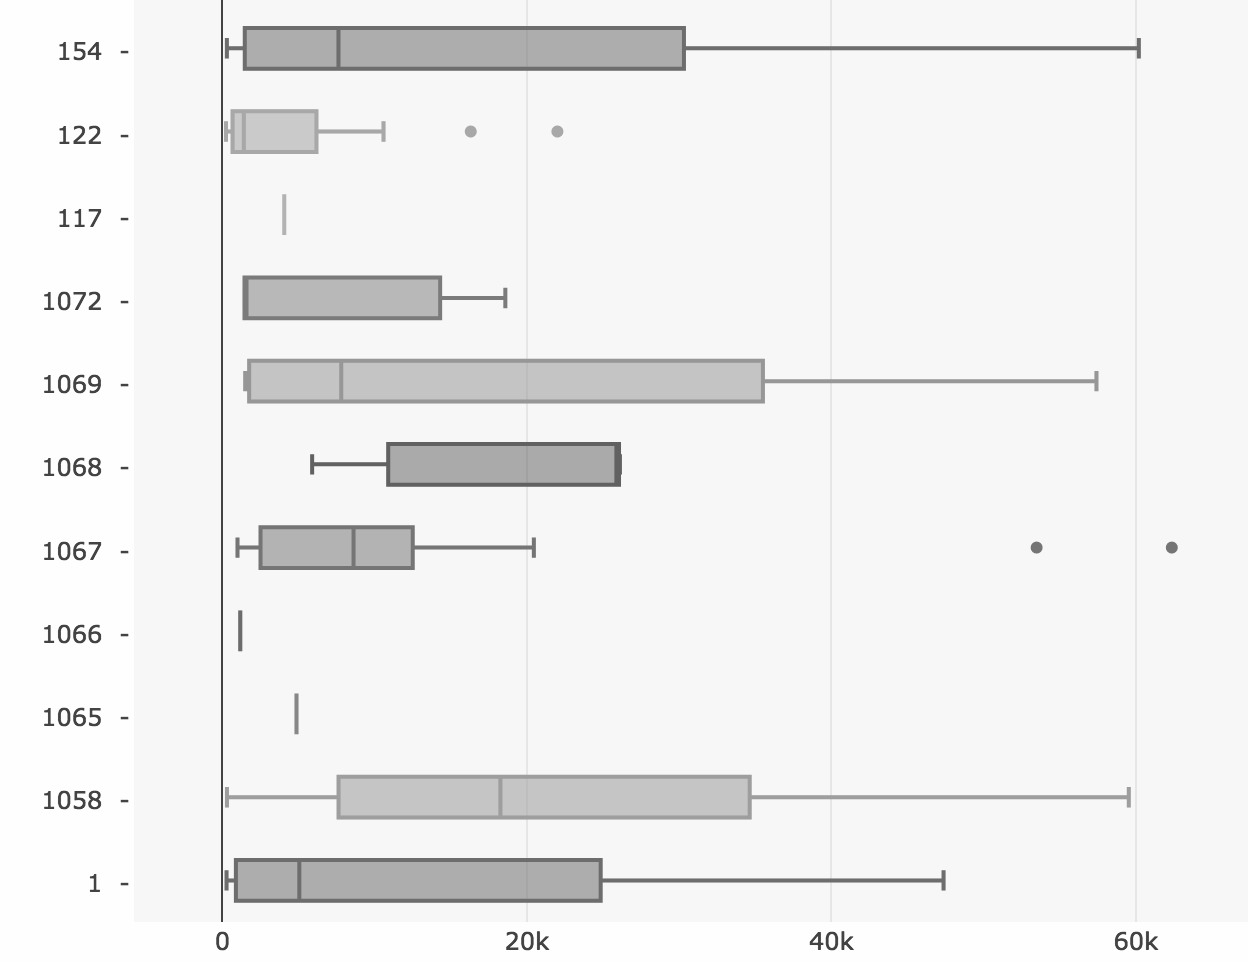
\includegraphics[width=0.4\linewidth]{time_per_user}
  \caption{The \epFeedItems shows a very high variability across users}
  \label{fig:tpu}
\end{figure*}
